\chapter{Application}
\label{cha:application}

In this chapter, we look at the effect of the optimisation techniques formulated in Chapter~\ref{cha:main_contributions} on different Agda code samples. Through a series of examples, we will see the effect of these optimisations and the degree to which they can yield increases in efficiency for both memory allocation space and execution time.

\section{Simple Module}

\input{Figures/Agda/latex/Example1}

Take for example the simple usage of record projections in Figure~\ref{code:example1_agda}. When we compile this module once without \texttt{-{}-inline-proj} on, and once again with \texttt{-{}-inline-proj} enabled, a unified diff of the two generated Haskell files gives us what is shown in Figure~\ref{fig:Example1_inline}.

\begin{figure}[h!]
    \centering
    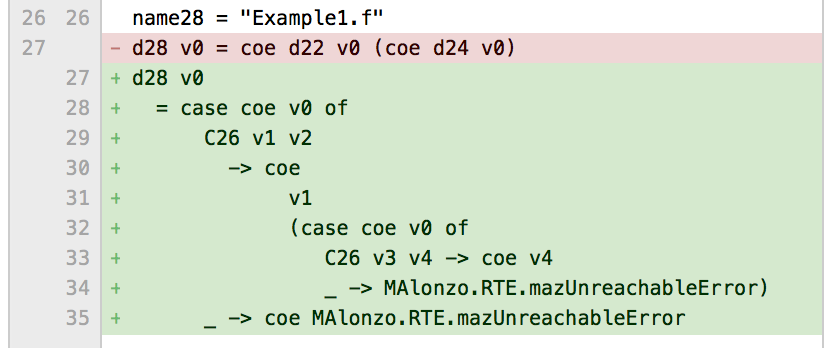
\includegraphics[width=0.5\textwidth]{Figures/Example1_inline}
    \caption{Unified difference of the \AgdaModule{Example1}~module compiled without and then with \texttt{-{}-inline-proj}.}
    \label{fig:Example1_inline}
\end{figure}

The compiled projection function \AgdaField{Pair.snd}, that is \lstinline{d18} in the Haskell code, is replaced with a Haskell expression that cases on the pair (\AgdaFunction{p} in Agda, \lstinline{d22} in Haskell) and returns the second field.

\begin{figure}[h!]
    \centering
    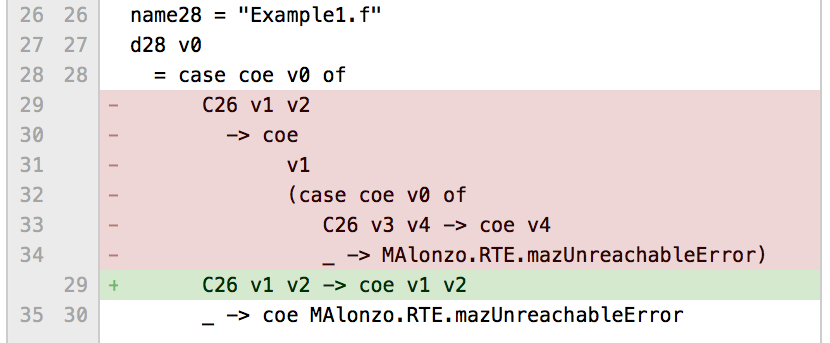
\includegraphics[width=0.5\textwidth]{Figures/Example1_squash}
    \caption{Unified difference of the \AgdaModule{Example1}~module compiled  with \texttt{-{}-inline-proj} and then also with \texttt{-{}-squash-cases}.}
    \label{fig:Example1_squash}
\end{figure}

We then compile the same file with both \texttt{-{}-inline-proj} and \texttt{-{}-squash-cases}, and the difference between only inlining and both inlining and squashing can be seen in Figure~\ref{fig:Example1_squash}.

\begin{figure}[h!]
    \centering
    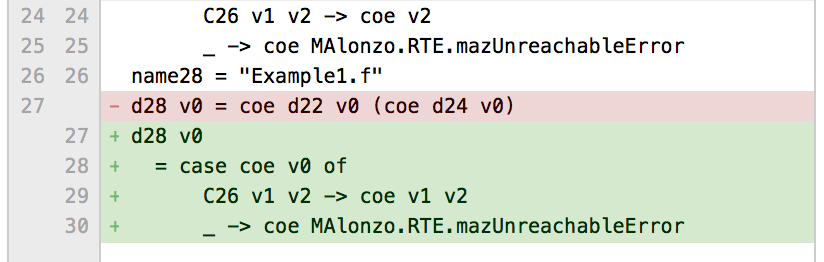
\includegraphics[width=0.5\textwidth]{Figures/Example1_inline_squash}
    \caption{Unified difference of the \AgdaModule{Example1}~module compiled without either optimisation, then with both \texttt{-{}-inline-proj} and \texttt{-{}-squash-cases}.}
    \label{fig:Example1_inline_squash}
\end{figure}

Figure~\ref{fig:Example1_inline_squash} shows the overall unified diff from neither optimisation to both.

\section{Triangle Module}

Triangle3sPB gives us an sample usage of mathematical pullbacks, by constructing triangle-shaped graphs and products of those graphs, as an example. These types of computations are relevant and important in many graph-rewriting calculations and can benefit from our optimisations.

When we compile this module once without \texttt{-{}-ghc-generate-pattern-let} on, and once again with \texttt{-{}-ghc-generate-pattern-let} enabled, a unified diff of the two generated Haskell files gives us what is shown in Figure~\ref{fig:Triangle_genplet}. Both times, the module was compiled with \texttt{-{}-inline-proj}.

\begin{figure}[h]
    \centering
    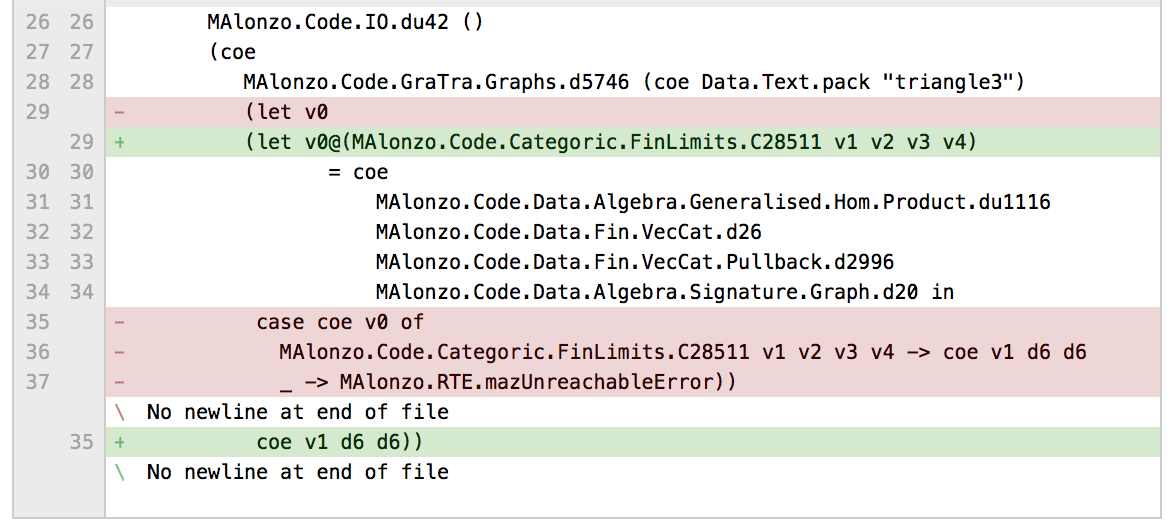
\includegraphics[width=0.5\textwidth]{Figures/Triangle_genplet}
    \caption{Unified difference of the \AgdaModule{Triangle3sPB}~module compiled without and then with \texttt{-{}-ghc-generate-pattern-let}.}
    \label{fig:Triangle_genplet}
\end{figure}

As is shown by this difference, the case analysis on \lstinline{v0} is no longer required and instead the constructor parameters are immediately bound in the enclosing \lstinline{let} expression.

\section{RATH-Agda Main}
\label{sec:app_one}

RATH-Agda is a basic category and allegory theory library developed by Kahl, et al.\citep{Kahl-2017_RATH-Agda-2.2} It includes theories relating to semigroupoids, division allegories, typed Kleene algebras and monoidal categories, among other topics.\citep{Kahl-2017_RATH-Agda-2.2} The RATH-Agda repository also provides a set of test cases in a \AgdaModule{Main} module, which can be used to test a variety of typical uses of the library's functions.

\subsection{Before}

In profiling the runtime of this \AgdaModule{Main} module, we found that an inordinate amount of time was spent on evaluating simple record projections. The first few lines of the profiling report in Figure~\ref{fig:main_prof} indicate that the greatest cost centres in terms of time are the two simple record projections for the $\Sigma$ data type, with a combined 17.6\% of execution time spent evaluating them.

Because enabling profiling does have an affect on execution, we also re-compiled the module without profiling and ran it six times, measuring execution time with the Unix \texttt{time} command, to determine its average runtime as 1.60 seconds.

\begin{figure}
\begin{verbatim}
        Time and Allocation Profiling Report  (Final)

           Main +RTS -S -H7G -M7G -A128M -p -RTS

        total time  =        6.75 secs   (6755 ticks @ 1000 us, 1 processor)
        total alloc = 1,300,428,688 bytes  (excludes profiling overheads)

COST CENTRE                                                 %time %alloc

Data.Product.Σ.proj₂                                         10.4    0.0
Data.Product.Σ.proj₁                                          7.2    0.0
Categoric.KleeneCategory.DirectSum.SumStar.Square.E⋆′         4.9    7.0
Data.SUList.ListSetMap.RawLSM.RawLSM3.RawLSM3-comp.comp       4.1   10.4
Data.SUList.ListSetMap.RawLSM.RawLSM3.RawLSM3-comp.comp₀      3.9    3.7
...
\end{verbatim}
\caption{Profiling report for RATH-Agda's \AgdaModule{Main} module, compiled without projection inlining.}
\label{fig:main_prof}
\end{figure}


\subsection{After}

By compiling \AgdaModule{Main} with our new option, \texttt{-{}-inline-proj}, enabled, we reduced total runtime and memory allocation, as can be seen by comparing Figure~\ref{fig:main_inline_prof} and Figure~\ref{fig:main_prof}.

We again re-compiled the module without profiling and ran it six times, measuring execution time with the Unix \texttt{time} command, to determine its average runtime with projections inlined as 1.44 seconds. We therefore produced a speedup of 1.11$\times$.

\begin{figure}[h!]
\begin{verbatim}
        Time and Allocation Profiling Report  (Final)

           Main +RTS -S -H7G -M7G -A128M -p -RTS

        total time  =        5.26 secs   (5261 ticks @ 1000 us, 1 processor)
        total alloc = 1,299,709,408 bytes  (excludes profiling overheads)

COST CENTRE                                                 %time %alloc

Data.SUList.ListSetMap.FinRel.Utils.FinId                     6.2    8.6
Data.SUList.ListSetMap.RawLSM.RawLSM3.MapImage.mapImage₀      5.6    5.5
Data.SUList.ListSetMap.RawLSM.RawLSM3.RawLSM3-comp.comp       4.9    8.8
Categoric.KleeneCategory.DirectSum.SumStar.Square.E⋆′         4.7    6.6
Data.SUList.ListSetMap.Semigroupoid.LSMJoinOp.\               3.8    8.3
...
\end{verbatim}
\caption{Profiling report for RATH-Agda's \AgdaModule{Main}~module, compiled with projection inlining enabled.}
\label{fig:main_inline_prof}
\end{figure}

